\section{Encoding Session Types in TypeScript}
% Design choices

Developers can implement their application using APIs generated from the EFSM
to guarantee correctness by construction.
Our approach integrates the EFSM into the development workflow by encoding
session types as TypeScript types.
Communication over the WebSocket protocol introduces additional constriants: 
communication is always initiated in the front-end and driven by user interactions, 
whilst back-end roles can only accept connections.
This motivates our design of encoding the session types differently for server (\cref{section:server}) and client (\cref{section:browser}) targets.

\fz{I think there is an important thing to note here, ``Server'' side is
  basically the side which accepts the connection and ``Client'' side is the
side which makes the connection. But this is orthogonal to whether it runs on
Node or on browser? (Correct me if I'm wrong)}

\am{Not for the case of WebSockets, because only WebSocket clients on browser can initiate connections and only WebSocket Server on Node can accept; will make this distinction clear.}

\subsection{Server-side API generation}
\label{section:server}

% Francisco: mention that it corresponds to the messages for the Noughts and Crosses example too

\begin{wrapfigure}{r}{0.5\textwidth}
  \vspace{-5mm}
  \begin{center}
    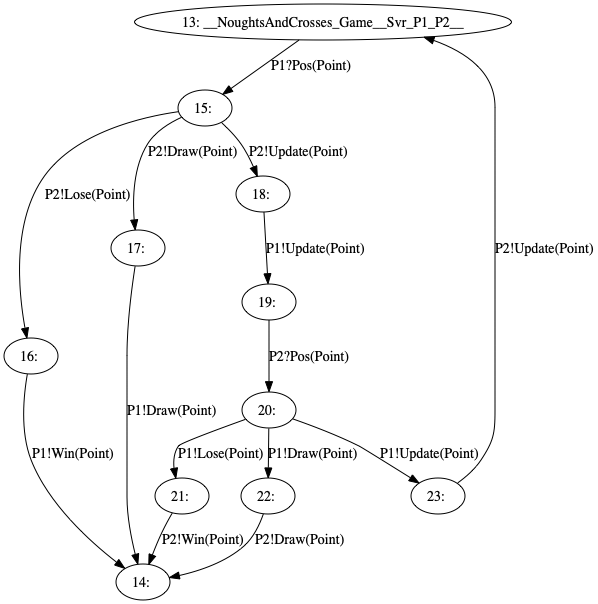
\includegraphics[width=0.48\textwidth]{figures/efsm_svr.png}
  \end{center}

  \vspace{-5mm}
  \captionof{figure}{EFSM for \texttt{Svr}.}
  \label{fig:efsmsvr}
\vspace{-1cm}
\end{wrapfigure}

We refer to the \texttt{Svr} EFSM (\cref{fig:efsmsvr}) as a running example in
this section.
For server-side targets, we encode EFSM states into TypeScript types and
consider receive and send states separately.
Each TypeScript encoding is assigned to its state identifier from the EFSM as
its type alias, thus providing syntactic sugar when referring to the successor
state in the TypeScript encoding of the current state.
For any state $S$ in the EFSM, we refer to the TypeScript type alias of its
encoding as $\llbracket S \rrbracket$.

\paragraph{Branching state}
We consider a receive state as a unary branching state for conciseness.
A branching state is encoded as an \textit{object literal}
\cite{TypeScriptSpec}, with each branch $i \in I$, $I$ denoting set of all
branches, corresponding to a member field.
A branch expecting to receive a message labelled $\texttt{label}_i$ carrying
payload of type $\texttt{T}_i$ with successor state $S_i$ is encoded as an
\textit{member field} named $\texttt{label}_i$ of function type
$(payload:\texttt{T}_i) \to \llbracket S_i \rrbracket$.
The developer implements a branching operation by passing callbacks for each
branch, parameterised by the expected message payload type for that branch.

\paragraph{Selection state}
We consider a send state as a unary selection state for conciseness.
A selection state is encoded as a \textit{union type}
\cite{TypeScriptSpec} of internal choice encodings: each internal choice $i \in
I$, $I$ denoting set of all choices, sending a message labelled
$\texttt{label}_i$ carrying payload of type $\texttt{T}_i$ with successor state
$S_i$ is encoded as a \textit{tuple type} of \texttt{[Labels.label$_i$, T$_i$,
  $\llbracket S_i \rrbracket$]}.
The developer implements a selection operation by passing the selected label
and payload to send in the message.
We generate a \textit{string enum} (named \texttt{Labels}) wrapping the labels
in the protocol.

\begin{figure}[ht]
\begin{lstlisting}[language=JavaScript]
export type S13 = { Pos: (payload: Point) => S15 };
export type S15 = [ Labels.Lose, Point, S16 ]
                | [ Labels.Draw, Point, S17 ]
                | [ Labels.Update, Point, S18 ];
\end{lstlisting}
\captionof{lstlisting}{Example encodings from \textit{Noughts and Crosses} \texttt{Svr} EFSM.}
\label{lst:svr}
\end{figure}

We make a key design decision \textit{not} to expose communication channels in
the TypeScript session type encoding to provide \textit{static} linearity
guarantees (\cref{section:serverlinear}).
Our encoding sufficiently exposes seams for the developer to inject their
business logic, whilst the generated session API
(\cref{section:serversessionapi}) handles the sending and receiving of
messages;
as a result, the encoding does not concern with the role involved in the
send/receive action. We outline the encoding below using examples from the
\textit{Noughts and Crosses} game (\cref{lst:svr}).

\subsubsection{Session runtime}
\label{section:serversessionapi}

Our session runtime performs communication in a protocol-conformant manner, but
does not expose these IO actions to the developer by delegating the
aforementioned responsibilities to an inner class.
The runtime listens to message (receive) events on the communication channel,
invokes the corresponding callback to obtain the value to send next, and
performs the send.
The developer instantiates the session by constructing an instance of the
session runtime class, providing the WebSocket endpoint URL (to open the
connection) and initial state (to execute the EFSM).

\subsubsection{Linear channel usage}
\label{section:serverlinear}
Channel linearity is guaranteed based on the correctness of our library design
and session runtime implementation, which means a faulty implementation could
violate this, but is up to the library author to verify once rather than the
end user. Our library design prevents the two properties below:

\paragraph{Repeated use}
We do not expose channels to the developer, which makes \textit{reuse}
impossible.
For example, to send a message, the generated API only requires the payload
that needs to be sent, and the session runtime performs the send internally,
guaranteeing this action is done \textit{exactly once} by construction.

\paragraph{Unused}
The initial state must be supplied to the session runtime
constructor in order to instantiate the session;
this initial state is defined
in terms of the successor states, which in turn has references to its
successors and so forth.
This encoding approach covers the terminal state (if it exists), and the
session runtime guarantees this terminal state, if it exists, will be reached
by construction.

\subsection{The React Framework}
Our browser-side session type encodings for browser-side targets build upon the React framework, developed by Facebook \cite{React} for the \textit{Model-View-Controller} (MVC) architecture. React is widely used in industry to create scalable single-page TypeScript
applications, and we intend for our proposed workflow to be beneficial in an
industrial context.
We introduce the key features of the framework.

\paragraph{Components}
A component is a reusable UI element which
contains its own markup and logic.
Components implement a \texttt{render()} function which returns a React
element, the smallest building blocks of a React application, analogous to the
view function in the MVU architecture.
Components can keep \textit{state} and the \texttt{render()} function is
invoked upon a change of state.
A simple counter can be implemented as a component,
with \texttt{count} stored as state, a button which increments \texttt{count}
when clicked and a \texttt{div} that renders the current
\texttt{count}.
Components can also render other components, which gives rise
to a parent/child relationship between components.
Parents can pass data to children as \textit{props} (short for properties).
Going back to the aforementioned example, the counter component could
render a child component \texttt{<StyledDiv count=\{this.state.count\} />} in
its \texttt{render()} function, propagating the \texttt{count} from its state
to the child.
This enables reusability, and for our use case, gives control to the parent
on what data to pass to its children (e.g. pass the payload of a received
message to a child to render).

\fz{Is VDOM needed to be covered here?}

\am{Intended to motivate how the session runtime implementation renders the required state and the VDOM deals with the diffs - at the same time, unsure whether this is important for the reader to understand (or just leave the DOM rendering as a black box)?}
\paragraph{Virtual DOM (VDOM)}
React components are rendered on a logical
abstraction of the DOM, which in turn performs a \texttt{diff} on the current
browser DOM and patches the delta accordingly.
This allows the developer to
directly specify what should be rendered without having to worry about which
elements to append or remove from the browser DOM.

\subsection{Browser-side API generation}

\label{section:browser}

\begin{wrapfigure}{r}{0.4\textwidth}
  \begin{center}
    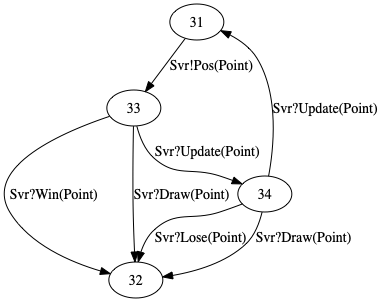
\includegraphics[width=0.4\textwidth]{figures/efsm_p1.png}
  \end{center}

  \captionof{figure}{EFSM for \texttt{P1}.}
  \label{fig:efsmp1}
\end{wrapfigure}

We refer to the \texttt{P1} EFSM (\cref{fig:efsmp1}) as a running example in
this section.
Preserving behavioural typing and channel linearity is challenging
for browser-side applications due to EFSM transitions being triggered by user
events:
in the case of \textit{Noughts and Crosses}, once the user makes a move by
clicking on a cell on the game board, this click event must be deactivated
until the user's next turn, otherwise the user can click again and violate
channel linearity.
Our design goal is to enforce this statically through the generated APIs.

For browser-side targets, we extend the approach presented in \cite{MVU2019} on
\textit{multiple model types} motivated by the \textit{Model-View-Update} (MVU)
architecture.
Each state in the EFSM is a \emph{model type} and uniquely defines a
\textit{view function}, set of \textit{messages} and \textit{update function}:
the view function defines what to render to the DOM, the set of messages define
the possible (IO) actions available at that state, and the update function
defines which successor state to transition to, given some supported IO action
at this state.

\subsubsection{Model types in React}

\paragraph{State}
An EFSM state is encoded as an \textit{abstract} React
component.
This is an abstract class to require the developer to provide their
own view function, which translates conveniently to the \texttt{render()}
function of React components.
Our session runtime (\cref{section:clientruntime}) ``executes'' the EFSM and
renders the current state.
Upon transitioning to a successor state, the successor's view function will be
invoked, as per the semantics expressed in \cite{MVU2019}.

\paragraph{Model transitions}
Transitions are encoded as React component props onto the encoded states by the
session runtime (\cref{section:clientruntime}).
We motivate the design choice of not exposing channel resources to provide
guarantees on channel usage.
React components in TypeScript are
\textit{generic} \cite{TypeScriptSpec}, parameterised by the permitted
types of prop and state.
The parameters allow us to leverage the TypeScript compiler to
verify that the props for model transitions stay local to the state they are
defined for.
The model transitions for EFSMs are message send and receive.

\subparagraph{Send}
We make the assumption that message sending is triggered by
some user-driven UI event (e.g. clicking a button, pressing a key on the
keyboard) which interacts with some DOM element.
We could pass a
\texttt{send()} function as a prop to the sending state, but the developer
would be free to call the function multiple times which makes channel reuse
possible.
Instead, we pass a \textit{factory function} as a prop, which will,
given an HTML event and a event handler function, return a fresh React
component that binds the sending action on construction.
So once the bound event is triggered, our session runtime executes the event
handler function to obtain the payload to send, perform the send
\textit{exactly once} and transition to (which, in practice, means render) the
successor state.

\begin{figure}[!h]
\begin{lstlisting}[language=JavaScript, tabsize=4]
// Inside some render() function..
{board.map((row, x) => (
	row.map((col, y) => {
		const SelectPoint = this.props.Pos('click', (event: UIEvent) => {
			event.preventDefault();
			return { x: x, y: y };}
		return <SelectPoint><td>.</td></SelectPoint>;
});}
\end{lstlisting}
\captionof{lstlisting}{Model transition for message sending in
\textit{Noughts and Crosses} \texttt{P1} implementation.}
\label{lst:clientapp}
\end{figure}

We demonstrate the semantics using the \textit{Noughts and Crosses} example in
\cref{lst:clientapp}.
\texttt{this.props.Pos} is the factory function prop
passed from the session runtime.
For each x-y coordinate on the game board, we
create a \texttt{SelectPoint} React component from the factory function (which
reads ``build a React component that sends the \texttt{Pos} message with x-y
coordinates as payload when the user clicks on it'') and we wrap a table cell
(the game board is rendered as a HTML table) inside the \texttt{SelectPoint}
component to bind the click event on the table cell.

\subparagraph{Receive}
The payload of a message receive transition is passed as
a prop to the successor state and can be handled in the successor's view
function.
Upon a message receive event, the session runtime renders the
successor of the receive state and propagates the payload to the successor
accordingly.

\subsubsection{Session runtime}
\label{section:clientruntime}

The session runtime can be interpreted as an abstraction on top of the React
VDOM that implements the EFSM by construction.
The session runtime itself is a React component too, named after the endpoint
role identifier:
it opens the WebSocket connection to the server, keeps track of the current
EFSM state as part of its React component state, and most importantly, renders
the React component encoding of the active EFSM state.
Channel communications are managed by the runtime, which allows it to render
the successor of a receive state upon receiving a message from the channel.
Similarly, the session runtime is responsible for passing the required props
for model transitions to EFSM state React components.
The session runtime component is rendered by the developer and requires, as
props, the \textit{endpoint URL} (so it can open the connection) and a list of
\textit{concrete state components}.

The developer writes their own implementation of each state (mainly to
customise how the state is rendered and inject business logic into state
transitions) by extending the abstract React class components.
The session runtime requires references to these concrete components in order to
render the user implementation accordingly.

\subsubsection{Affine channel usage}
A limitation of our browser-side session type encoding is only being able to
guarantee that channel resources are used \textit{at most once} as supposed to
\textit{exactly once}.

Communication channels are not exposed to the developer so multiple sends are
impossible.
This does not restrict the developer from binding the send action to exactly
one UI event: for \textit{Noughts and Crosses}, we bind the \texttt{Pos(Point)}
send action to each unoccupied cell on the game board, but the generated
runtime ensures that, once the cell is clicked, the send is only performed once
and the successor state is rendered on the DOM, so the channel resource used to
send becomes unavailable.

However, our approach \textit{does not} statically detect whether all
transitions in a certain state are bound to some UI event.
This means that it is possible for an implementation to \textit{not} handle
transitions to a terminal state but still type-check, so we cannot prevent
unused states. Equally, our approach does not prevent a client closing the browser, which would drop the connection.
